\section{Crossover Operators}
\label{sec:crossover}

This chapter gives a general overview of the different variations of crossover operators. There exists a great number of different crossover operators which have been developed for different specific problems. In this chapter, we will concentrate not only on crossover operators specifically designed for the TSP but we will also discuss some other operators which were used in the literature for other optimization problems. \par 

Section \ref{subsec:opx},  introduces a classical one-point crossover (OPX). In Section \ref{subsec:path_crossovers}, we introduce path representation crossovers and illustrate how they work on examples. Section \ref{subsec:adjacency_crossovers} focuses on adjacency representation crossovers providing the examples of the corresponding approaches. Note that each example generates only one offspring. The second offspring can be generated by switching the roles of two parent chromosomes. Finally, Section \ref{subsec:edge_recombination} introduces the edge recombination crossover (ERX).\par

\subsection{One-Point Crossover}
\label{subsec:opx}

One-point crossover (\textbf{OPX}) was developed by \citeauthor{holland1975adaptation} \cite{holland1975adaptation} to work with chromosomes which were represented as bit strings. Two parent chromosomes are cut at a randomly chosen position. The part before the cut point is taken from the first parent chromosome while the part after the cut point is taken from the second parent chromosome. \par 
For instance, we have the first parent chromosome 110100 and the second parent chromosome 000111. Let 1 be our randomly chosen cut point. This means that the substring 11 is taken from the first parent, and the substring 0111 is taken from the second parent. The resulting offspring is 110111 (see Figure \ref{fig:6_1_OP}). 

\begin{figure}[htp] \centering
	\centering
	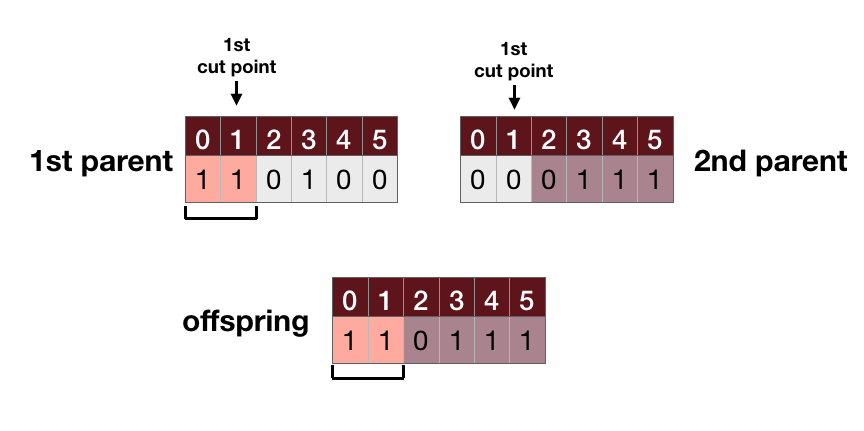
\includegraphics[width=0.6\textwidth]{6_1_OP}
	\caption{One-point crossover between parent chromosomes 110100 and 000111 in bit-string representation.}
	\label{fig:6_1_OP}
\end{figure}

This crossover operator always produces valid offsprings for the TSP only in the ordinal representation which was pointed out in Section \ref{subsec:ordinal}. For instance, let 02000 be the first parent chromosome in the ordinal representation which corresponds to 03124 in the path representation. Then, let 00210 be the second parent chromosome in the ordinal representation which corresponds to 01432 in the path representation. Let 1 be a randomly chosen cut point. The resulting offspring is 02210 which corresponds to 03421 in the path representation (see Figure \ref{fig:6_1_OP_Ordinal}). \par 
 
 \begin{figure}[htp] \centering
 	\centering
 	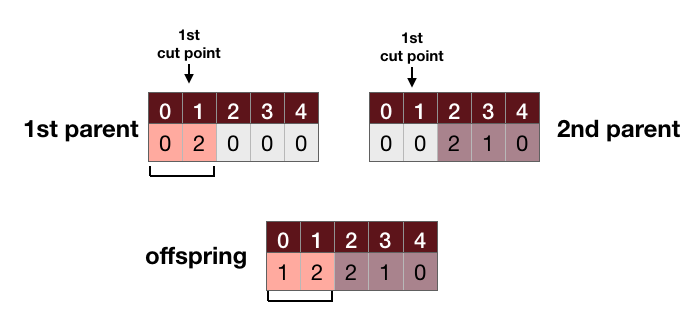
\includegraphics[width=0.6\textwidth]{6_1_OP_Ordinal}
 	\caption{One-point crossover between parent chromosomes 02000 and 00210 in ordinal representation.}
 	\label{fig:6_1_OP_Ordinal}
 \end{figure}
 
However, this crossover operator cannot be used directly for the TSP in the path and adjacency representation because simply exchanging parts of the parent chromosomes mostly results in invalid offsprings (see Figure \ref{fig:6_1_OP_invalid_for_tsp}). Therefore, some transformations of this operator are required, where the validity of the offspring is guaranteed. As a result, a great number of other crossover operators has been proposed which achieve this goal. We are going to discuss them in the following sections. \par 

\begin{figure}[htp] \centering
	\centering
	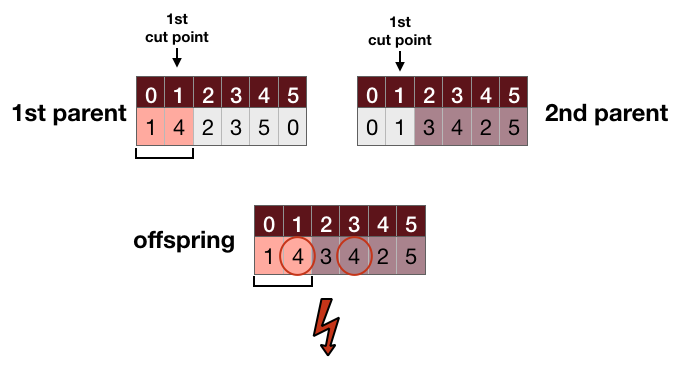
\includegraphics[width=0.6\textwidth]{6_1_OP_invalid_for_tsp}
	\caption{One-point crossover between parent chromosomes 142350 and 013425 in path representation for the TSP.}
	\label{fig:6_1_OP_invalid_for_tsp}
\end{figure}

\subsection{Path Representation Crossovers}
\label{subsec:path_crossovers}

The crossover operators of this type work with the chromosomes which encapsulate a tour in the path representation. These crossover operators differ mainly in the way of preserving the order of the cities from the parent chromosomes. Some of them preserve the absolute positions and the others preserve the relative order. The crossover operators of these group are:

\begin{itemize}
	\item Crossover operators preserving absolute positions:
		\subitem Partially-mapped crossover, 
		\subitem Cycle crossover. 
	\item Crossover operators preserving relative order:
		\subitem Modified crossover,
		\subitem Order crossover,
		\subitem Linear order crossover,	
		\subitem Order-based crossover,  
		\subitem Position-based crossover.
\end{itemize}

Please note that we also consider this classification for our experiments: We will analyze whether any of these groups performs generally better than the other.

\subsubsection{Partially-Mapped Crossover }
\label{subsubsec:pmx}

\begin{figure}[htp] \centering
	\centering
	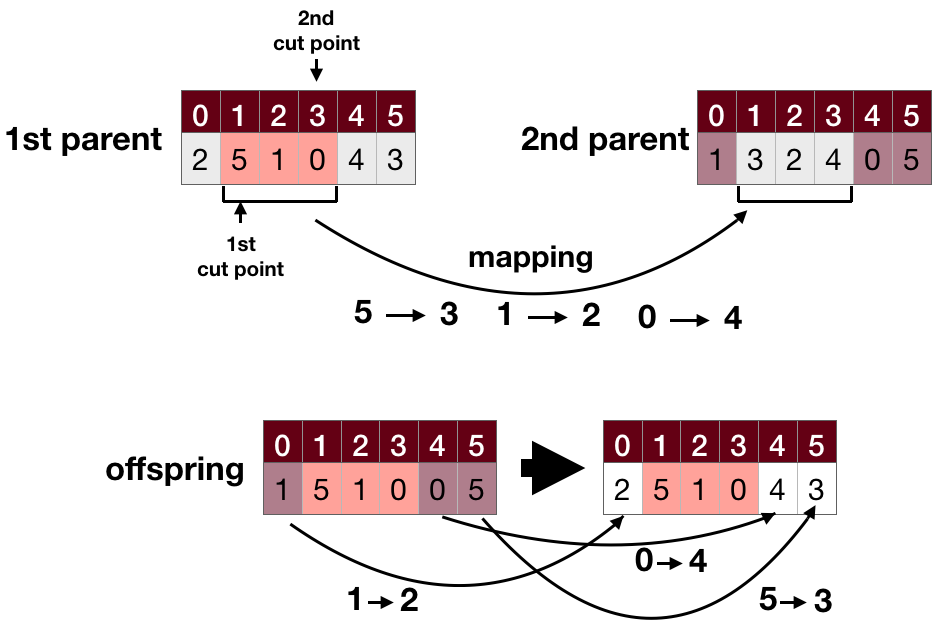
\includegraphics[width=0.6\textwidth]{partially-mapped_crossover}
	\caption{Partially-mapped crossover between parent chromosomes 251043 and 132405.}
	\label{partially-mapped_crossover}
\end{figure}

Partially-mapped crossover (\textbf{PMX}) as discussed by \citeauthor{potvin1996genetic} \cite{potvin1996genetic} takes two cut points. The cities which stand between these cut points in the first parent chromosome go directly to the offspring at exactly the same positions. The remaining positions are filled with the cities from the second parent chromosome. In order to handle possible duplicates, a mapping between two parents chromosomes for the region between the two cut points is introduced. \par

Consider for instance the example from Figure \ref{partially-mapped_crossover} with parent chromosomes 251043 and 132405. Let us assume that the two cut points are 1 and 3. This means that the substring 510 of the first parent is directly copied into the offspring. When filling in the remaining positions based on the second parent, we get the offspring chromosome \mbox{1 510 05}. To eliminate the duplicates we make a mapping between the elements between the cut points in the parents chromosomes: 510 is mapped to 324, i.e., 5 is mapped to 3, 1 is mapped to 2, and 0 is mapped to 4.  When applying this mapping, we replace 1 with 2 in the offspring at the position 1 and get 251005. As we see, the updated chromosome is not final as 0 is duplicated as well, therefore it will be replaced by 4 according to the mapping and we get 251045. Now we have to deal with the last 5 which can be replaced by 3. As a result we get the offspring 251043. \par

One can also think of this procedure as applying two mappings to the second parent: First, a mapping $m$ is applied for replacing the positions between the cut points. In our example, $m$ is defined as follows: $3 \rightarrow 5$, $2 \rightarrow 1$, $4 \rightarrow 0$. That is, the sequence $324$ in the second parent is replaced by $510$. Afterwards, the mapping $m$ is inverted, giving us $m^{-1}: 5 \rightarrow 3$, $1 \rightarrow 2$, $0 \rightarrow 4$. This inverse mapping is then applied to all remaining positions.\par

Multiple replacements at the same position can occur if both parents have the same city in the part of the tour between the chosen cut points. Consider for instance the example from Figure \ref{partially-mapped_crossover_mult_replacements} with the first parent chromosome 051243 and the second parent 125430. Let the two cut points be 1 and 3.  In this case, 5 is mapped to 2, 1 is mapped to 5 and 2 is mapped to 4. Again the part between the chosen cut points from the first parent (512) goes directly to the offspring at the same positions, whereas the rest is taken from the second parent. As a result, we get the offspring 1 512 30. The city 1 is duplicated in the offspring, so it will be replaced by another value according to the defined mapping, namely by 5. Now the offspring consists of 5 512 30. However, the city 5 is duplicated as well and is replaced by 2, resulting in the offspring \mbox{2 512 30}. The city 2 is, however, duplicated as well, therefore another replacement will be made. The city 2 is replaced by 4 according to the mapping. As the cities 3 and 0 are not duplicated, no replacements are necessary. The resulting offspring is 4 512 30. 

\begin{figure}[htp] \centering
	\centering
	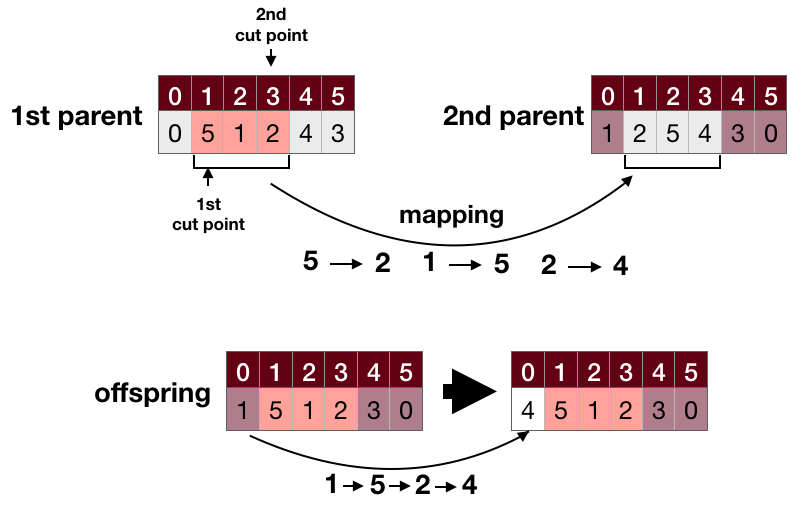
\includegraphics[width=0.6\textwidth]{partially-mapped_crossover_mult_replacements}
	\caption{Partially-mapped crossover with multiple replacements between parent chromosomes 051243 and 125430.}
	\label{partially-mapped_crossover_mult_replacements}
\end{figure}

\subsubsection{Cycle Crossover} 
\label{subsubsec:cycle}

Cycle crossover (\textbf{CX}) as discussed by \citeauthor{potvin1996genetic} \cite{potvin1996genetic} looks for a cycle in the two parent chromosomes. A cycle consists of a set of cities which are found in the same set of positions in both parent chromosomes. For instance, let the first parent chromosome have the genes 0543162 and the second parent chromosomes have the genes 0435216. The set of cities $\{3,4,5\}$ is found in the same set of positions in both parents (namely $\{1,2,3\}$), constituting a cycle 5-4-3-5 (see Figure \ref{cycle_crossover}). 

\begin{figure}[htp] \centering
	\centering
	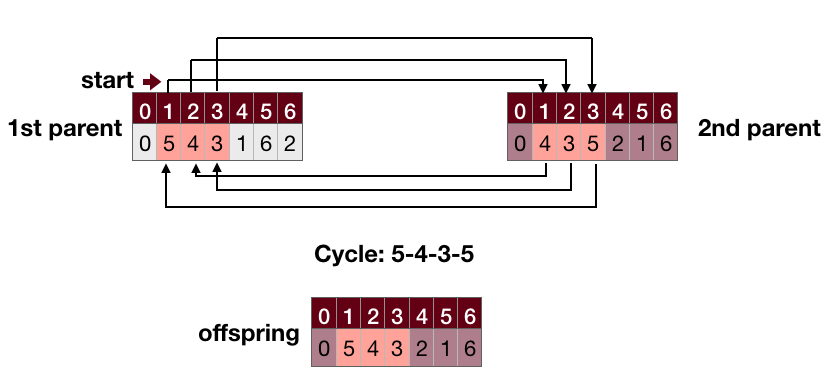
\includegraphics[width=0.7\textwidth]{cycle_crossover}
	\caption{Cycle crossover between parent chromosomes 0543162 and 0435216.}
	\label{cycle_crossover}
\end{figure}

To find a cycle, we start from the index where the parent chromosomes differ from each other. In our example, this means that we ignore the city 0 which occupies the same position 0 in both parents, as it will not make any changes to the offspring. So we start with the index 1, where the city 5 is found in the first parent. Then we look for a city which stands at the same index in the second parent chromosome. In our case it is the city 4. Then we look for the index in the first parent chromosome where this city stands. It is index 2. We find the city in the second parent chromosome which stands at this index as well, namely the city 3. Now we go to the first parent chromosome and see that the city 3 stands there at the index 3. In the second parent, the city 5 occupies the position 3 and we found a cycle 5-4-3-5. \par

The cities of this cycle are copied from the first parent chromosome to the offspring and occupy the same positions there. All the remaining positions are filled with the cities from the second parent chromosome at exactly the same positions. As a result, the position of each city in the offspring is inherited from one of the parents and the resulting offspring is 0543216. Therefore, each element comes from one parent together with its position.\par

Alternatively, to find a cycle we could start at a random index and not at the beginning. Moreover, instead of just filling the remaining positions of the offspring with the cities from the second parent, we could search for additional cycles and use them to populate the offspring. Consider the example from Figure \ref{cycle_crossover_mult_cycles} with the parent chromosomes 051463278 and 042315687. The first element is the same in both parents, so the city 0 goes directly to the offspring to the position 0. Here we have  three cycles, namely 5-4-3-5, 1-2-6-1, 7-8-7. So, at first, the subset of cities $\{3,4,5\}$,which corresponds to the first cycle, goes to the offspring at the positions from the first parent. Then the subset of cities $\{1,2,6\}$, which corresponds to the second cycle, goes to the offspring at the positions from the second parent. Finally, the subset $\{7,8\}$ goes to the offspring at the positions from the first parent again, resulting in the offspring 052413678.

\begin{figure}[htp] \centering
	\centering
	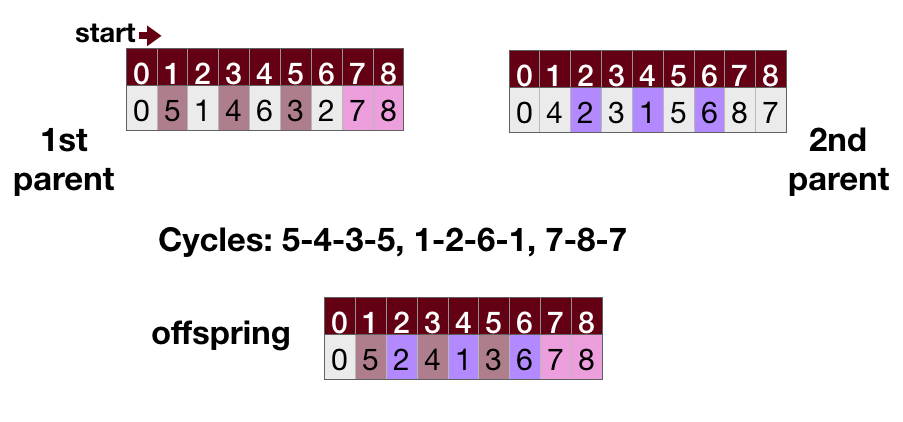
\includegraphics[width=0.7\textwidth]{cycle_crossover_mult_cycles}
	\caption{Cycle crossover while using multiple cycles between parent chromosomes 051463278 and 042315687.}
	\label{cycle_crossover_mult_cycles}
\end{figure}

\subsubsection{Modified Crossover}
\label{subsubsec:modified}
Modified crossover (\textbf{MX}) as introduced by \citeauthor{davis1985applying} \cite{davis1985applying} randomly chooses an index, at which the first parent chromosome will be cut into half. 
The cities before the cut point are taken from the first parent and go to the offspring at the same positions. The other indices of the offspring are filled with the cities from the second parent, starting at the beginning of the second parent chromosome. In order to avoid duplicates, the next city goes from the second parent to the offspring, only if this city has not been taken from the first parent chromosome yet. Otherwise, this city is ignored and the next city from the second parent goes to the offspring.\par

\begin{figure}[htp] \centering
	\centering
	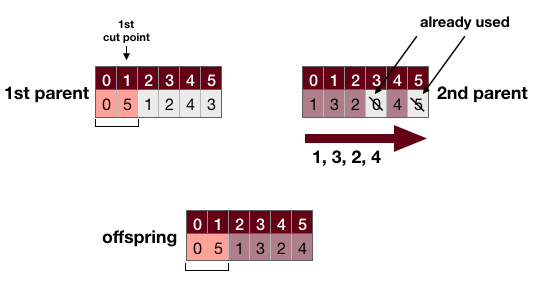
\includegraphics[width=0.7\textwidth]{modified_crossover}
	\caption{Modified crossover between parent chromosomes 051243 and 132405.}
	\label{modified_crossover}
\end{figure}

For instance consider Figure \ref{modified_crossover}, where the first parent chromosome is 051243 and the second parent chromosome is 132045. Let the cut point be the index 1. Then, the cities which stand in the first parent before this cut point, namely 0 and 5, go directly to the offspring at the same positions. Now the cities from the second parent starting from its beginning are used: The city 1 goes to the offspring at the next free index, namely the index 2. So do the cities 3 and 2. The next city 0 has been already taken from the first parent chromosome, therefore it will be not used and the next city is taken into consideration, namely the city 4, which goes to the offspring at the last index. The last city 5 from the second parent has been already taken from the first parent, therefore we ignore it. The resulting offspring has the genes 051324.

\subsubsection{Order Crossover}
\label{subsubsec:order}

Order crossover (\textbf{OX}) as discussed by \citeauthor{potvin1996genetic} \cite{potvin1996genetic} takes two indices which correspond to two cut points. The part of the first parent chromosome between these indices is copied to the offspring directly at exactly the same positions. The other positions will be filled with the cities from the second parent chromosome in the following way: We start searching in the second parent at the index which stands just after the second cut point.  If the observed city has already been used, when the cities were copied from the first parent, it will be ignored and the next city is considered. If the end of the second parent chromosome is reached during the search, the search continues at the beginning of it and continues until the second cut point is reached.\par

\begin{figure}[htp] \centering
	\centering
	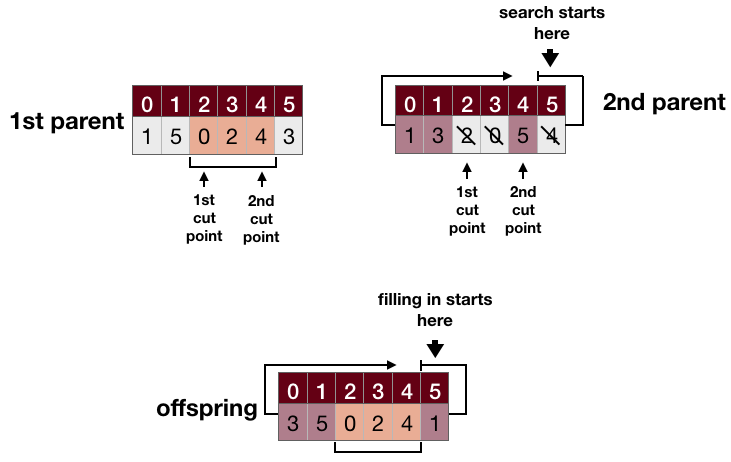
\includegraphics[width=0.6\textwidth]{order_crossover}
	\caption{Order crossover between parent chromosomes 150243 and 132054.}
	\label{order_crossover}
\end{figure}

For instance, consider the parent chromosomes 150243 and 132054 (see Figure \ref{order_crossover}). The chosen cut points are the indices 2 and 4. This means that the part of the first parent chromosome 024 goes directly to the offspring at the positions 2,3 and 4, respectively. Now the remaining part of the offspring will be filled. We start with the index after the second cut point and find the city 4 in the second parent chromosome. As this value has already been taken from the first parent chromosome, it cannot be used and the next city to be considered is the city 1 which stands at the index 0 in the second parent. This city has not been used yet, therefore it takes the position right after the second cut point, i.e. the position with the index 5, in the offspring. Now the end part of the offspring is full, therefore the next insertions continue at the beginning of the offspring chromosome, starting at the index 0. The next city in the second parent which is considered is the city 3. As it has not been used yet, it goes to the offspring at the position 0. The city 2 was already used, and so was the city 0. Then the city 5 is inserted at the position 1 in the offspring. Now, the second cut point in the parent chromosome is reached, and the offspring is filled. Therefore, the crossover is over, and the resulting offspring has the genes 350241.
\vspace{2cm}

\subsubsection{Linear Order Crossover}
\label{subsubsec:linear_order}

Linear order crossover (\textbf{LOX}) was used by \citeauthor{akay2013recent} \cite{akay2013recent} for the job shop scheduling problem. However, as this crossover operator works similar to the order crossover, which was discussed above, we will apply it to the TSP. The difference is that the remaining positions of the offspring are filled starting from the beginning of the offspring chromosome. Also the search of the next candidate city in the second parent  starts at the beginning of the second parent chromosome and continues sequentially until its end is reached.\par

We consider the example which was used above for order crossover with the first parent chromosome 150243, the second parent chromosome 132054 and the indices 2 and 4 (see Figure \ref{linear_order_crossover}). The offspring gets the genes 024 from the first parent at the positions 2,3 and 4, respectively. The remaining part of the offspring will be filled, starting with the first index 0. The candidate city for this position is searched in the second parent at the position 0, where the city 1 is found. As it has not been used in the offspring yet, it occupies the position 0 in the offspring. In the same way, the next city 3 from the second parent chromosome goes to the position 1 in the offspring. The positions 2 to 4 are already filled, therefore the next candidate from the second parent will go at the last index 5. And it will be the city 5, which can be taken into consideration in the second parent. Therefore, the resulting offspring has the genes 130245.
Note that this operator works exactly as the order crossover does, if the cut interval is chosen at the end of the chromosome.

\begin{figure}[htp] \centering
	\centering
	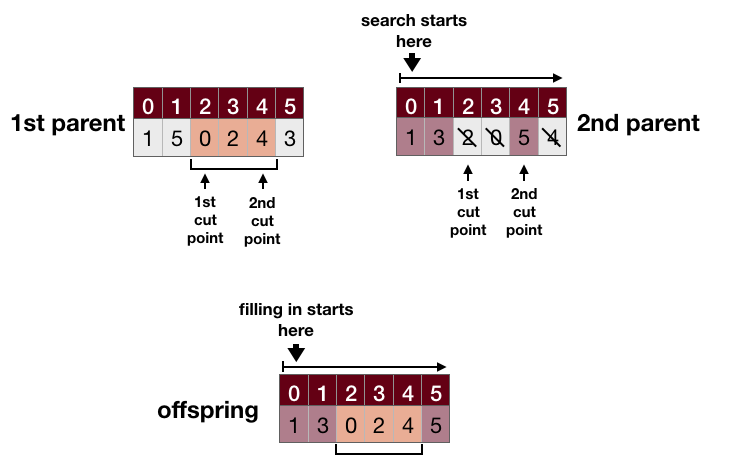
\includegraphics[width=0.6\textwidth]{linear_order_crossover}
	\caption{Linear order crossover between parent chromosomes 150243 and 132054.}
	\label{linear_order_crossover}
\end{figure}

\subsubsection{Order-Based Crossover}
\label{subsubsec:order_based}
Order-based crossover (\textbf{OBX}) as discussed by \citeauthor{potvin1996genetic} \cite{potvin1996genetic} randomly selects a subset of cities in the first parent chromosome and puts them into the offspring in exactly the same order in which these cities occur in the first parent, but at the positions, which these cities occupy in the second parent. Each remaining position in the offspring is filled with a city which occupies this position in the second parent. As a result, if the initial, randomly chosen subset of cities is very small, then the offspring is very similar to the second parent chromosome.\par

For instance, let the first parent chromosome be 051243 and the second parent chromosome be 132405 (see Figure \ref{order-based_crossover}). The chosen subset of cities is $\{3,4,5\}$. These cities appear in the first parent chromosome in the order 5, 4, 3. This order must be preserved. In the second parent, they occupy the positions 1, 3, 5. Therefore, these cities appear in the offspring in the defined order at the positions 1, 3, 5. The remaining positions are filled with the other cities from the second parent, preserving their positions. The resulting offspring has the genes 152403.

\begin{figure}[htp] \centering
	\centering
	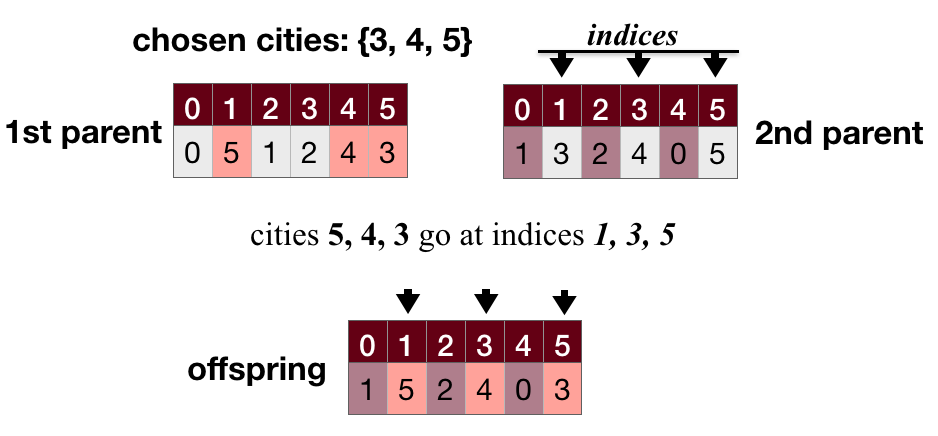
\includegraphics[width=0.6\textwidth]{order-based_crossover}
	\caption{Order-based crossover between parent chromosomes 051243 and 132405.}
	\label{order-based_crossover}
\end{figure}

\subsubsection{Position-Based Crossover}
\label{subsubsec:position_based}
Position-based crossover (\textbf{PBX}) as discussed by \citeauthor{potvin1996genetic} \cite{potvin1996genetic} takes randomly a subset of positions. The cities which occupy these positions in the first parent chromosome go directly to the offspring chromosome at the same positions. All the remaining positions of the offspring are filled with the cities from the second parent chromosome in the following way: Starting from the beginning of the second parent chromosome, the next city comes into consideration. If it was already taken from the first parent, then the city is ignored and the next city on the consecutive position comes into question. This operator therefore preserves the absolute order of the cities which are taken from the first parent chromosome and the relative order of the cities which are taken from the second parent chromosome.\par
For instance, take the parent chromosomes 150243 and 132054 (see Figure \ref{position-based_crossover}). The set of chosen positions is $\{1,3,4\}$. Cities 5, 2 and 4 occupy these positions in the first parent and are inserted into the offspring at these positions. Now the genes of the second parent chromosome are used. The city which occupies the starting position 0 in the second parent is the city 1. It has not been used yet, therefore, the city 1 goes to the offspring at the position 0. The next city in question is the city 3. It has not been used yet as well, therefore it occupies the next free position in the offspring, namely the position 2. The next two positions in the offspring are already filled. Therefore, the last position is filled with the city 0 from the second parent, which is the last city which has not been used yet.
So, the resulting offspring has the genes 153240.\par

\begin{figure}[htp] \centering
	\centering
	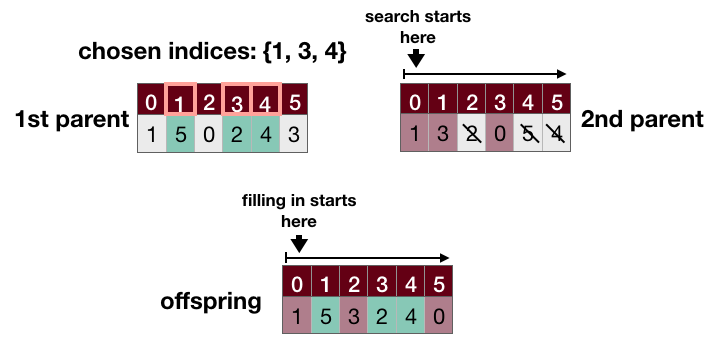
\includegraphics[width=0.6\textwidth]{position-based_crossover}
	\caption{Position-based crossover between parent chromosomes 150243 and 132054.}
	\label{position-based_crossover}
\end{figure}

Note that this crossover operator is similar to linear order crossover. The only difference is that the PBX takes a subset of positions instead of an interval in the first parent chromosome.\par

\subsection{Adjacency Representation Crossovers}
\label{subsec:adjacency_crossovers}
The main aim of the crossover operators using this type of tour representation is to preserve as many edges from the parent chromosomes as possible, as this information is relevant for the TSP. Together with the ERX (see Section \ref{subsec:edge_recombination}), these crossover operators are therefore called edge-preserving operators (see \cite{potvin1996genetic}). In each step, they use either an edge from the first parent chromosome or an edge from the second one. An exception is the last edge, which is normally not inherited from the parents but is added to the final solution in such a way that the Hamilton cycle is closed. \par

Please note that according to \citeauthor{potvin1996genetic} \cite{potvin1996genetic}, "the edge-preserving operators are superior to the other types of crossover operators".

\subsubsection{Alternate Edges Crossover}
\label{subsubsec:alternate_edges}

The alternate edges crossover (\textbf{AEX}) was described by \citeauthor{grefenstette1985genetic} \cite{grefenstette1985genetic}. It alternately chooses the edges from the two parents. It includes the following steps:

\begin{enumerate}
	\item Choose randomly an edge $(s, u)$ from one of the parents as a starting point for the child tour.
	\item Choose from the other parent an edge $(u, v)$ which is incident to the chosen edge $(s, u)$ and extend the tour.
	\item If the chosen edge introduces a cycle, choose a random edge which does not introduce a cycle and extend the tour.
	\item Extend the tour further by choosing the edges alternately from the parents until all the cities are included into the tour.	 
\end{enumerate}

For instance, we have the following parent tours: 123450 and 140532. Let us assume that the edge $(0, 1)$ was randomly chosen from the first parent. It will be directly copied into the child (see Figure \ref{alternate_edges_1}). The next edge $(1, 4)$, which is incident to the city 1, will be taken from the second parent and put into the child tour. The next edge $(4, 5)$ comes from the first parent. The next two edges are $(5, 2)$ and $(2, 3)$. They extend the tour, as it is shown in Figure \ref{alternate_edges_2}. The last edge is supposed to be taken from the second parent and it would be the edge $(3, 5)$. However, it introduces a cycle and cannot be taken (see Figure \ref{alternate_edges_3}).\par

Instead, the last possible edge $(3, 0)$ is chosen and finishes the tour. As this edge was the only possible edge to extend the tour, a random choice could not be applied in this case. The resulting offspring is 143052. According to \citeauthor{grefenstette1985genetic} \cite{grefenstette1985genetic}, the results of using this crossover were disappointing. Nevertheless, we include it as well in order to compare it to other crossovers.

\begin{figure}[htp] \centering
	\centering
	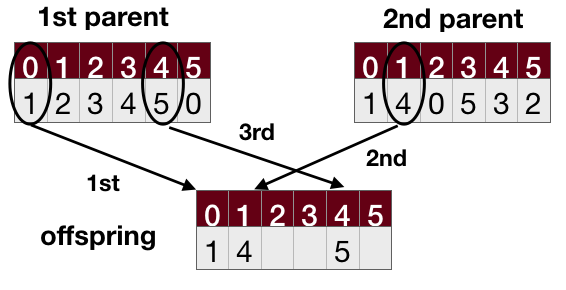
\includegraphics[width=0.5\textwidth]{alternate_edges_1}
	\caption{Alternate edges crossover: Introducing the edges (0, 1), (1, 4), (4, 5).}
	\label{alternate_edges_1}
\end{figure}

\begin{figure}[htp] \centering
	\centering
	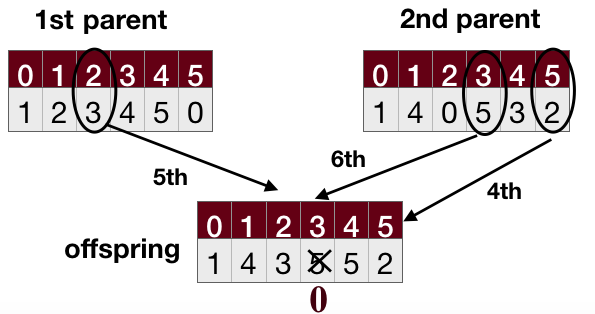
\includegraphics[width=0.5\textwidth]{alternate_edges_2}
	\caption{Alternate edges crossover: Introducing the edges (5, 2), (2, 3).}
	\label{alternate_edges_2}
\end{figure}

\begin{figure}[htp] \centering
	\centering
	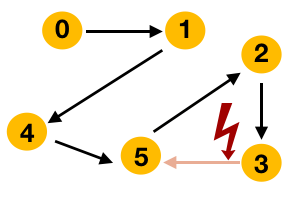
\includegraphics[width=0.2\textwidth]{alternate_edges_3}
	\caption{Alternate edges crossover: Cycle in the tour after adding the edge $(3, 5)$.}
	\label{alternate_edges_3}
\end{figure}
 
\subsubsection{Heuristic Crossover}
\label{subsubsec:heuristic}

The heuristic crossover (\textbf{HX}) was introduced by \citeauthor{grefenstette1985genetic} in \cite{grefenstette1985genetic} for improving the effectiveness of the genetic algorithm for the TSP. In general, genetic algorithms are free from domain information, which makes them widely applicable.  For better performance on a specific domain, a so-called "hybrid" genetic algorithm can be introduced, where some domain-dependent information is used. The heuristic crossover considers the distances on the edges and looks for the shortest parental edge to a city, which has not been visited yet. The HX algorithm includes the following steps:

\begin{enumerate}
	\item Choose randomly a city $s$ as a starting point for the child tour.
	\item Find an edge $(s, u)$ in the first parent and an edge $(s, v)$ in the second parent extending the tour from the current city $s$.
	\item Choose the edge with a smaller distance. If this edge leads to a cycle in the current partial tour, choose randomly an edge which does not introduce a cycle.
	 \item Go to step $2$ and continue to extend the current partial tour by choosing the shorter edge in the parents which extends the tour, until all the cities are included into the tour.	 
\end{enumerate}

 There exist some modifications to this algorithm. As discussed by \citeauthor{potvin1996genetic} \cite{potvin1996genetic}, both \citeauthor{liepins1987greedy} \cite{liepins1987greedy} and \citeauthor{suh1987incorporating} \cite{suh1987incorporating} proposed a modification of step $4$:
If the shortest parental edge leads to a cycle in the current partial tour, then the edge from the other parent will be used. If it also introduces a cycle, then extend the tour with a random edge that does not introduce a cycle. 

Let us again make an example. Consider the parent chromosomes 13420 and 14302 (see Figure \ref{hX}). Let us assume that the first edge was chosen at the index 0. As the 0th edge in the both parents is the same, the offspring gets this edge, i.e. 1 goes at the index 0. Now 1 is the next index. The edge $(1, 3)$ in the first parent has the distance 7, whereas the edge (1, 4) in the second parent has the distance 10 (see the distance table in Figure \ref{dist_table}). 

 \begin{figure}[htp] \centering
	\centering
	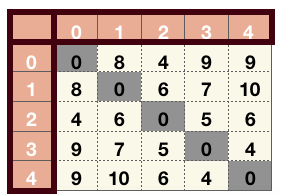
\includegraphics[width=0.3\textwidth]{dist_table}
	\caption{Distance table for the HX example in Figure \ref{hX}.}
	\label{dist_table}
\end{figure}

\begin{figure}[htp] \centering
	\centering
	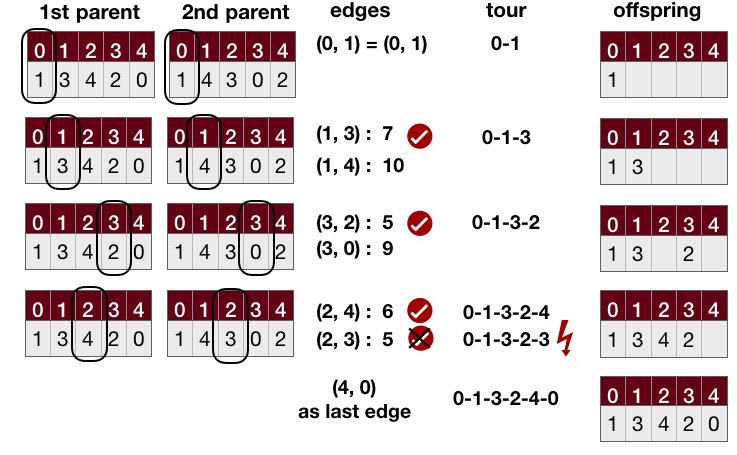
\includegraphics[width=\textwidth]{hX}
	\caption{Heuristic crossover for parent chromosomes 13420 and 14302.}
	\label{hX}
\end{figure}

Based on its smaller distance, we choose the edge from the first parent and check whether it leads to a subcycle. The current tour of the offspring with this edge is 013. We do not have a subcycle here; therefore, the edge $(1, 3)$ goes to the offspring. The next index is 3. The edge $(3, 2)$ in the first parent with distance 5 wins against the edge $(3, 0)$ in the second parent having a distance of 9. The current offspring is 13-2- which corresponds to the tour $\pi = (0, 1, 3, 2)$. The next index 2 brings us to the edge $(2, 4)$ in the first parent with distance 6 and to the edge $(2, 3)$ in the second parent with distance 5. The edge $(2, 3)$ wins but it introduces a subcycle 3-2-3. For this reason, the other edge $(2, 4)$ is taken and the current offspring with this edge is 1342-. There is no choice for the last edge because we need a Hamilton cycle. Thus, getting the last edge $(4, 0)$, the resulting offspring is 13420 which corresponds to the tour $\pi = (0, 1, 3, 2, 4)$. Please note that it is identical to the first parent.
 
It is interesting to note that this crossover tends to repeat one of the parents, if the number of genes is small.

\subsection{Edge Recombination Crossover}
\label{subsec:edge_recombination}
We consider the edge recombination crossover (\textbf{ERX}) developed by \citeauthor{whitley1989scheduling} \cite{whitley1989scheduling} separately because it combines the features of the previous two groups. On the one hand, it works with the path representation like the path representation crossovers do. On the other hand, its aim is to transfer as many parental edges to the offspring as possible like the adjacency representation crossovers do. For this reason, it uses a special data structure called 'edge map'. This edge map contains for each city a list of cities, which are the neighbors of this city either in the first parent or in the second parent chromosome. That is, it lists for each city all adjacent cities in both parents. \par

For instance, assume that we have two parent chromosomes 02314 and 31420 in the path representation (see Figure \ref{edge_map_initial}). The city 0 has the adjacent cities 2, 3, 4 in both parents. The list for the city 1 includes 3 and 4. The city 2 has the neighbors 0, 3, 4 and so on. 

\begin{figure}[htp] \centering
	\centering
	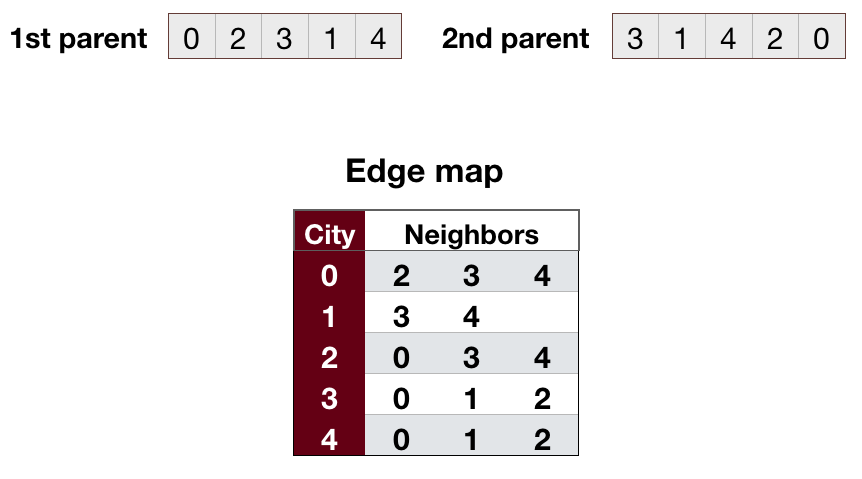
\includegraphics[width=0.4\textwidth]{edge_map_initial}
	\caption{Initial state of the edge map for the parent chromosomes 02314 and 31420.}
	\label{edge_map_initial}
\end{figure}

\begin{figure}[htp] \centering
	\centering
	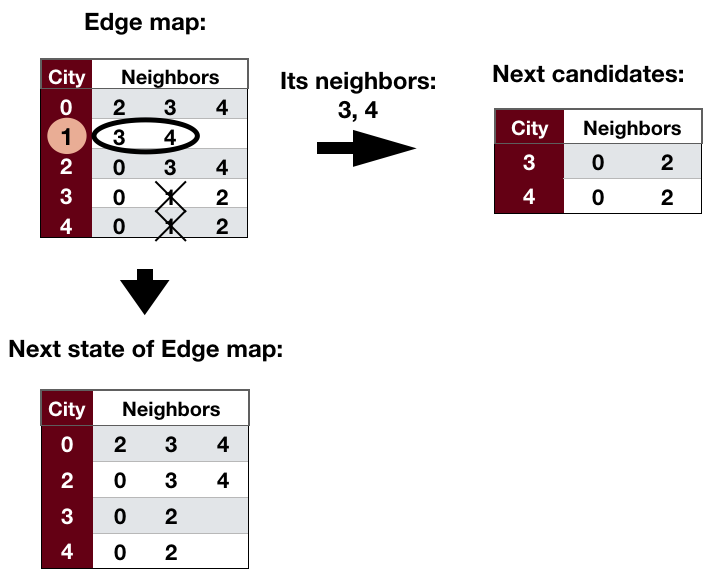
\includegraphics[width=0.5\textwidth]{Edge_map_after_city_chosen}
	\caption{State of the edge map for the parent chromosomes 02314 and 31420 after choosing the city 1.}
	\label{Edge_map_after_city_chosen}
\end{figure}

\begin{figure}[htp] \centering
	\centering
	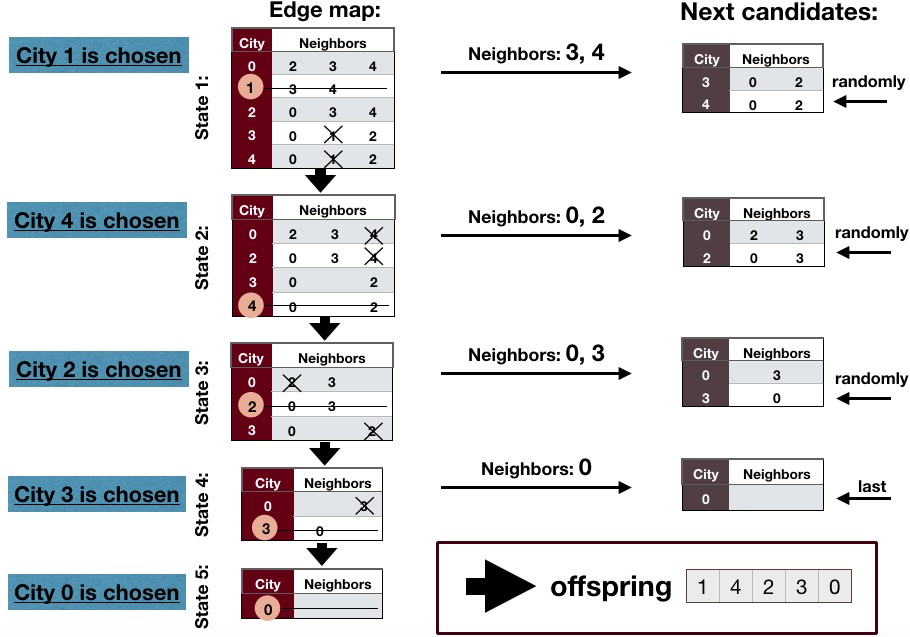
\includegraphics[width=\textwidth]{er}
	\caption{Edge recombination crossover for the parent chromosomes 02314 and 31420.}
	\label{er}
\end{figure}

This is the initial state of the edge map because no cities have been included in the offspring yet. All the edges in the edge map are called "active", as they are available to continue the tour. Among these, ERX chooses the edge which leads to a city with the minimal number of active edges. In other words, a city with the smallest list of neighbors will be chosen. If there is more than one candidate city, the choice is made randomly among them. The edge map will be updated after each city selection, so that only active edges stay there.\par

We will demonstrate how the edge recombination crossover works using the above mentioned parent chromosomes and the constructed edge map from Figure \ref{edge_map_initial}.\par 

The city with the shortest list of neighbors is the city $1$. So, it will be selected and added to the tour. This city has neighbors $3$ and $4$. Therefore, these cities will be now considered as the next candidates to continue the tour and the city $1$ will be deleted from the map (see Figure \ref{Edge_map_after_city_chosen}). Figure \ref{er} shows how the edge map transforms while doing this crossover. So, the next step is to compare  the candidates according to the length of their list of neighbors. The candidate with the shortest list will be chosen. If some candidates have lists of equal minimal length, as in our example the cities $3$ and $4$, then one of them will be taken randomly. Let us assume that the city $4$ was randomly chosen. It will be added to the tour and deleted from the edge map. As this city has the cities $0$ and $2$ as neighbors, they are the next candidates to continue the tour. Both cities have the same number of neighbors, therefore one of them will be chosen randomly. Let us assume that the city $2$ was chosen and is added to the tour. Its neighbors have the same number of neighbors as well; therefore, the city $3$ is assumed to be chosen randomly. This city continues the tour and its only neighbor, the city $0$, finishes the tour. The resulting offspring is 14230.\par